%
\documentclass[a4paper]{article}
\usepackage[utf8]{inputenc}
%~ \usepackage{fullpage}
\usepackage{amsmath,amssymb}
\usepackage[colorlinks]{hyperref} % use colored text in stead of ugly boxes
%~ \usepackage[toc]{multitoc} % Nice two-column TOC
\usepackage{pdfpages}
%~ \usepackage{pgf}
%~ \usepackage{tikz}


\title{Programming Life - Seminar report}

\author{
Group 5/E: 
 Felix Akkermans,  
Niels Doekemeijer, \\
Thomas van Helden, 
Albert ten Napel,
Jan Pieter Waagmeester 
}

\begin{document}

\maketitle

\begin{abstract}
\noindent For the  development of a modeling and simulation package for BioBricks we attended a seminar in synthetic biology, in which essential knowledge from this domain was gathered. Together with an abstract of the seminars, a reflection on the relationship of this project with synthetic biology is given, motivating the value of the effort that this project makes at applying computer science in the field of synthetic biology. Alongside of that we provide a reflection on which role computer science plays in biology in general.
\end{abstract}

\section{Abstracts of the seminar}
For each seminar a summary was made. This chapter provides an abstract of each summary in chronological order. The summaries themselves are provided in appendix~\ref{abstracts}.

\subsection{Introduction to molecular cell biology}
DNA is a molecule that provides the information for the construction of proteins. This molecule can be divided in several ways to provide pieces to describe the buildup of DNA. Messenger RNA (mRNA) relays the information in DNA to the protein synthesis machinery. mRNA shares a similarity with DNA, but is directly used in protein construction, because mRNA encodes for the amino acids that  make up the protein. In this chain of translation, there are several factors that play a role in promoting or suppressing this process. The expression of DNA varies based on the type of cell and the life form. Based on the study of this, the ability to influence this arises, and allows for manipulation of DNA and the partial prediction of it's outcome. 

\subsection{Math in biology}
The math in biology centers very much around the concentration of molecules in the cell or cell compartments. The concentration and the speed in which the concentration changes is determines by the speed of reactions that create or break down the molecules. These interactions can be modeled using differential equations. Because of the interaction between these organic molecules, some processes are catalyzed and others surpressed. Enzymes play a big role in this and the reactions between them are described by enzyme kinetics. With these models that describe the expression and interaction between genes, gene networks can be imagined and described in genes. By placing these in a cell, bacterial response regulators or activators can be used to target promoters or suppressors. This way, input from outside the cell can be provided to these gene networks, to create a information processing system. Such systems can implement signal generating components or logical gates.

\subsection{iGEM contest}

To motivate students and bring advances in synthetic biology, the iGEM contest challenges teams from universities all around the world to create and study systems in synthetic biology.

The team from University Groningen attempted to tackle a problem in the watersupply of areas where it is unsure whether the water is polluted. To determine this pollution they implemented a mechanism in E. Coli to detect certain pollutants and create a visible reaction. The aim is to change the buoyancy of the cell by producing gas, so it will float to the surface.

The team of Imperial College London created a framework for biosensors. Their aim was to create better reaction biosensors, so they react faster and more noticeable. For this they modified \textit{B. subtilis}, and as an example made it reacting to a harmful substance, so that it is visible for the human eye. This could be applied to detect contaminated water.

The aim of Cambridge was to create glowing \textit{E. Coli} that produces a large amount of light. For this the bioluminescence in fireflies and several light producing bacteria. These processes were optimized and adapted for \textit{E. Coli}. Maximizing the light production by ten times brought new insights on the application of this.

\subsection{Bioinformatics}
The increase in data that biology produced opened a lot of possibilities in analysis. Among fields of interests are the properties of genes, the prediction of the functioning of genes, research on the relation of genes among species, the integration of databases with biological information, and the search for molecules that could serve a wanted purpose. In medicine, this knowledge opens up the possibility for personalized treatment based on your genome. Other trends are analysis of RNA-splicing, and the development of a sort of \textit{web 2.0} for bioinformatics to share the knowledge.

\section{Relationship between this project and synthetic biology}

In computer science, one could argue that programming lies at the very foundation. Since the discovery of DNA in biology, the knowledge about its working gave the insights on how DNA translates to complex effects and behaviour very similar as to a programming language. Analogous to how the simple languages in computer programming that spawned great complexity in this field of science gave raise to the demand of tools to aid this development, this  also goes for DNA in biology. And this parallel with computer science makes it inviting to use the same methods and paradigms, to build layers of abstraction and functionality.

In this project, we attempt to apply a selection of paradigms of computer science, and use some of the technologies that have proven to be successful in computer science, and bring them in the field of synthetic biology. The migration of these to a field of science that is quite a foreign domain for computer science deserves careful implementation and an open mind to new problems.

We will create a modelling and simulation package for BioBricks. The power of a modelling and simulation suite has significantly aided and accelerated the development of numerous technologies in computer science and other fields, and the aim is to bring these same benefits to those working beyond the border between computer science and biology. This will apply  biological  math to model the functioning of biological systems, and a GUI and simulation server environment in modern, mature technologies from computer science.

\section{The role of computer science in biology}
Computer science came about not with the purpose to study itself. It was a means to and end, an aid to accelerate technology and fields of science where it could be applied at the time. Biology was not a big user of this concept at first. Since the discovery of DNA and the development of technologies to read and synthesize these, together with the development of technologies to observe and analyse molecular processes such as cells, the bandwidth of digital data that biology produces constantly exploded. This is where computers came in. Computers are ideal for processing large amounts of data. But computers have some cathing up to do. We think that in order to do this, biology should not have to walk the same path as other fields did and work with antique technologies, but should immediately benefit from the latest improvements in computer science. We also think that the marriage of computer science and biology holds a very exiting future with its application in society, and with a lot of potential which will probably spawn a lot of new fields in science. We think it could very well play a key role in solving the most important problems humanity is and will be facing. This fusion of two fields of science could greatly determine the shape of our future. We therefore think that it deserves special attention. This could be in the form of contests to motivate students to pick up this field, or consciousness raising of the general public to create more support for this field among policy makers.
\appendix

\section{Seminar summaries}
\label{abstracts}
Here the summary of each seminar is given in chronological order.

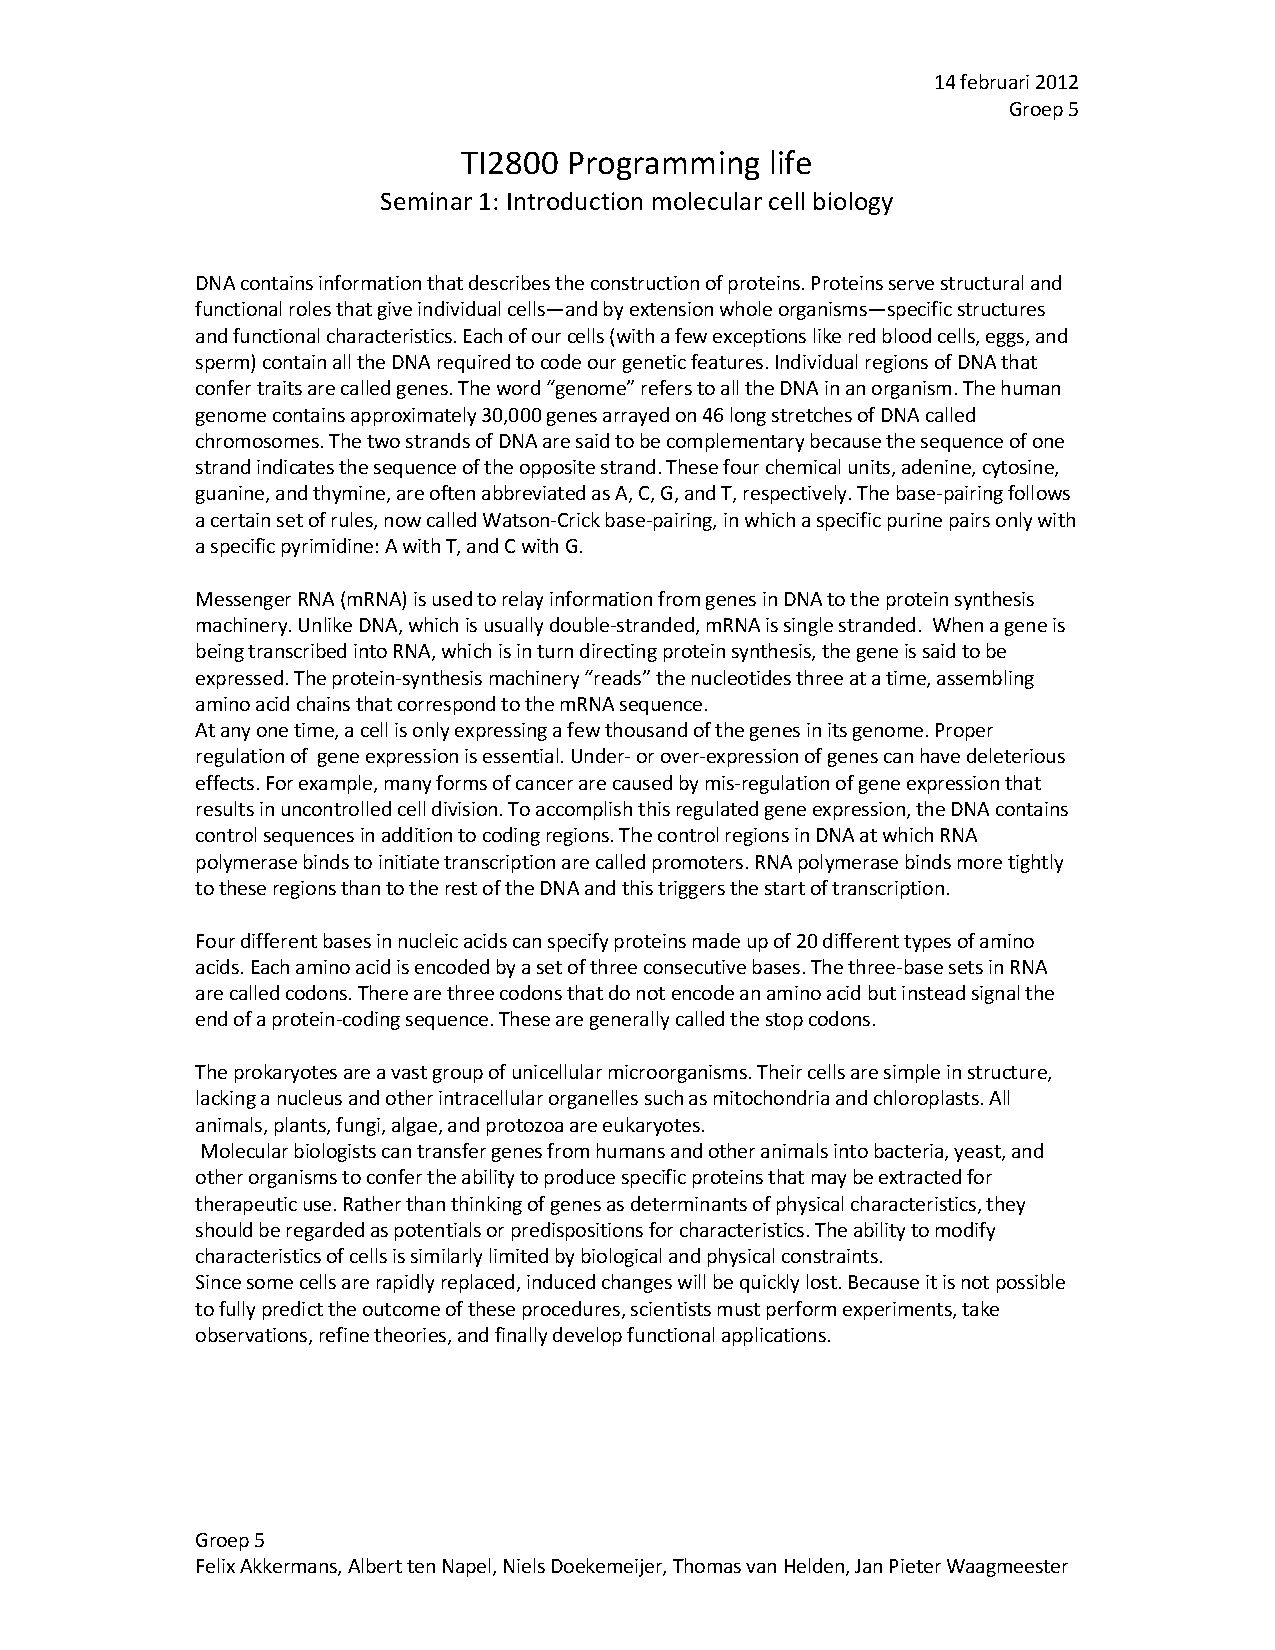
\includepdf{abstracts/lecture-1.pdf}
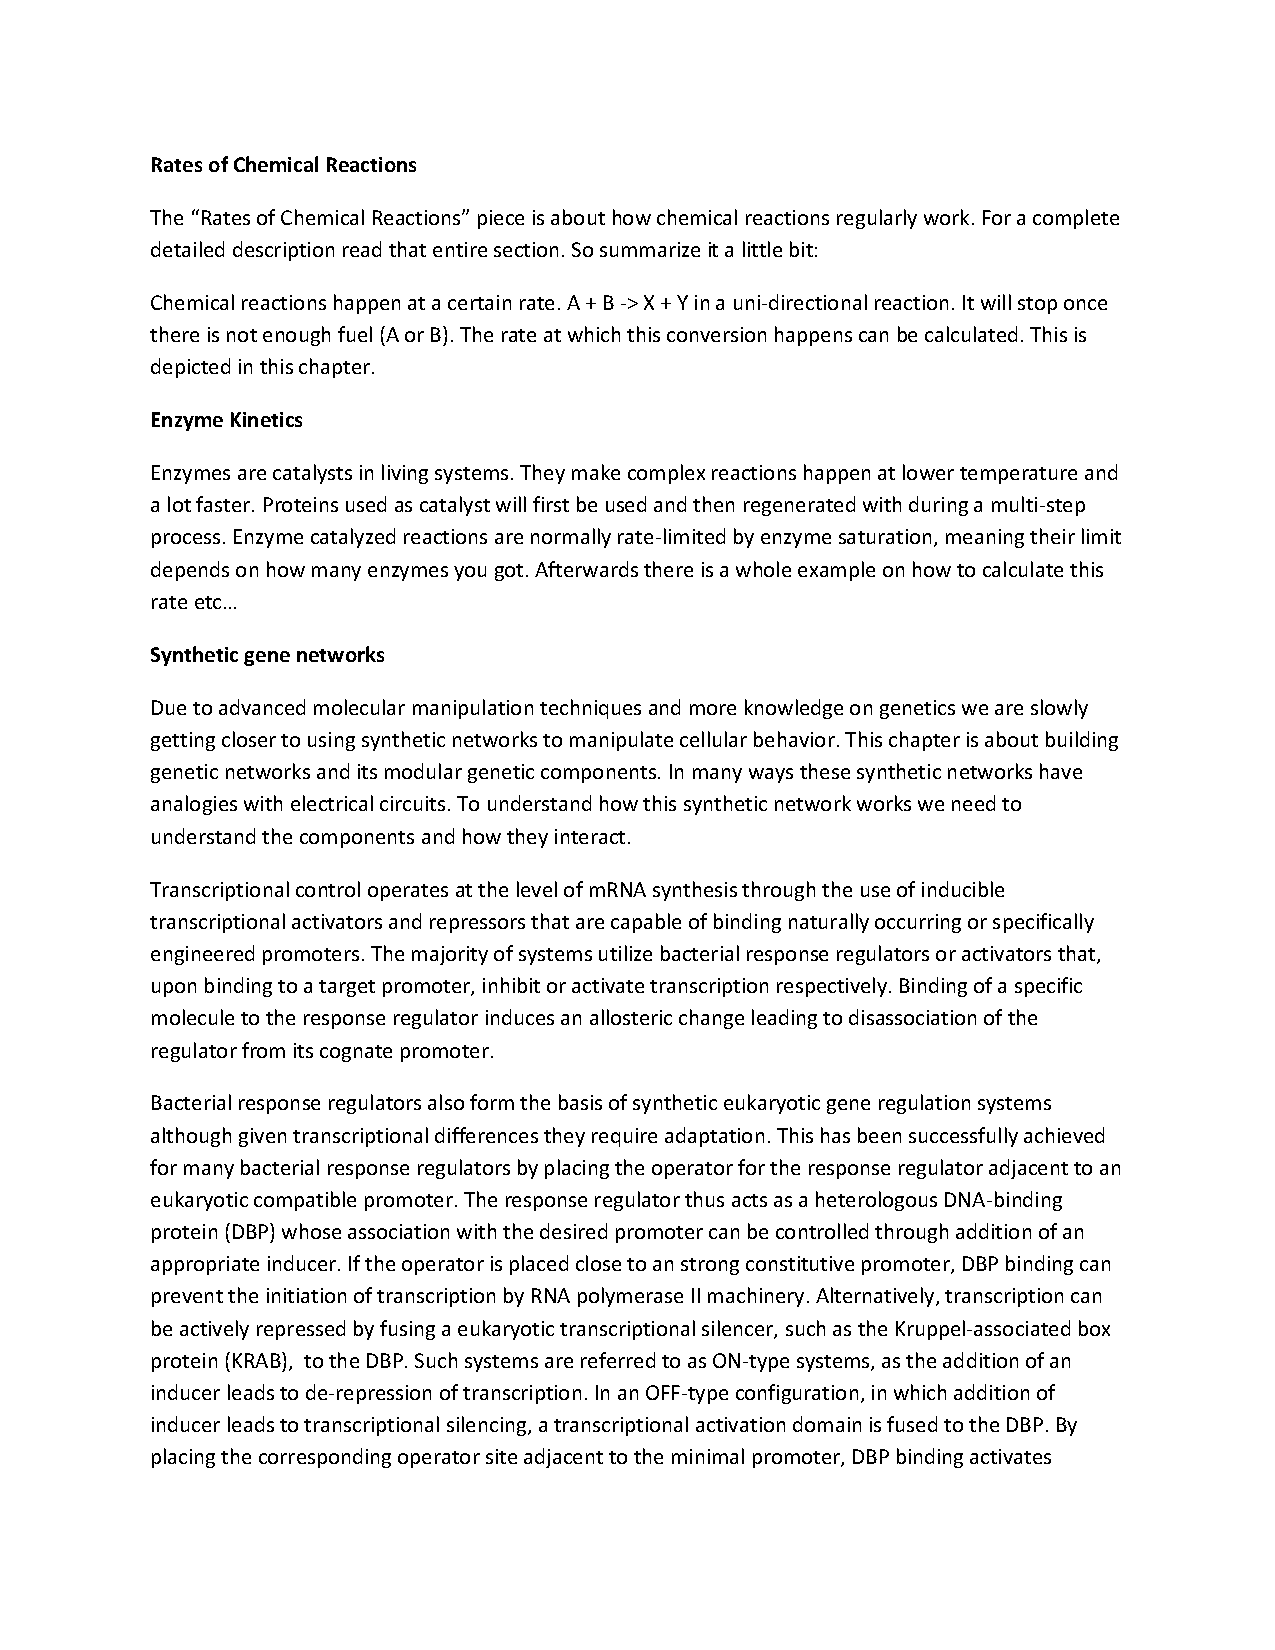
\includepdf{abstracts/lecture-2.pdf}
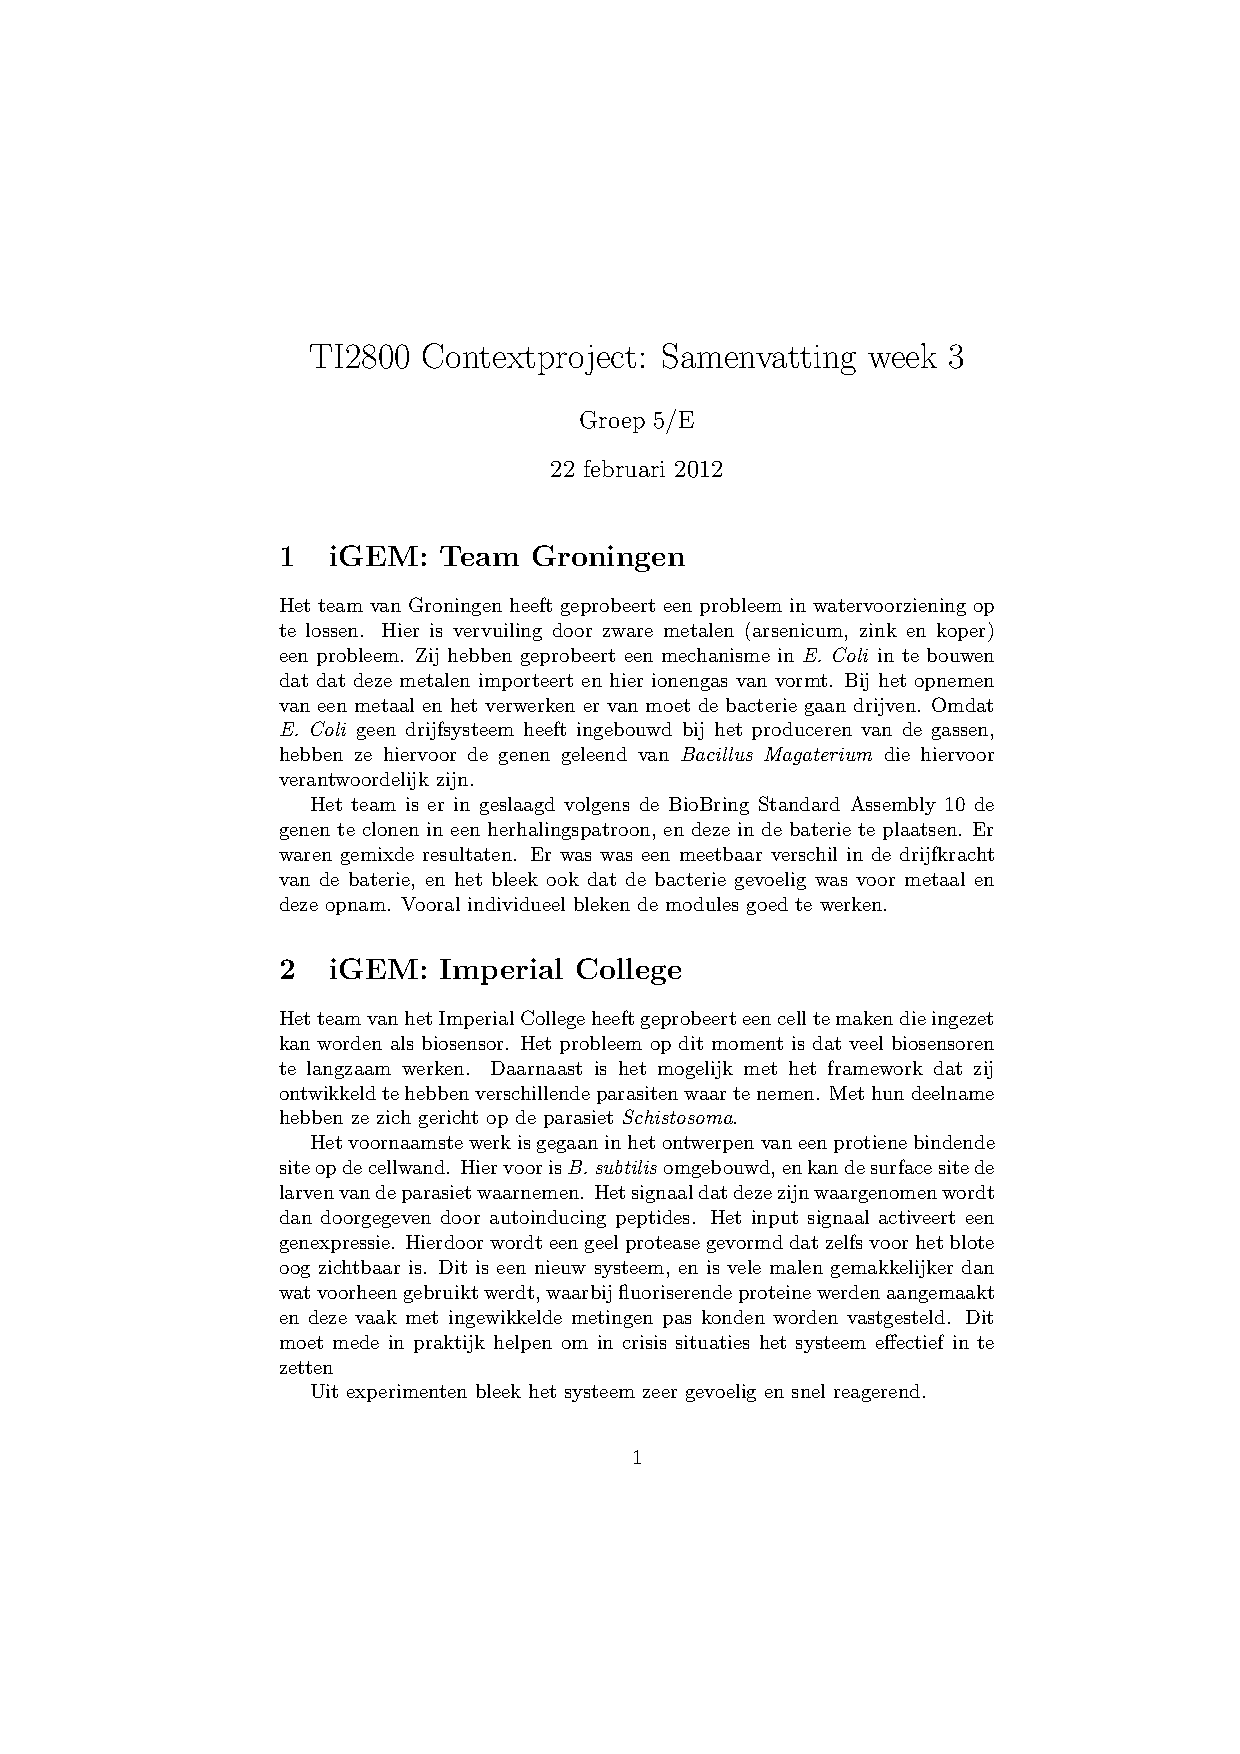
\includepdf{abstracts/lecture-3.pdf}
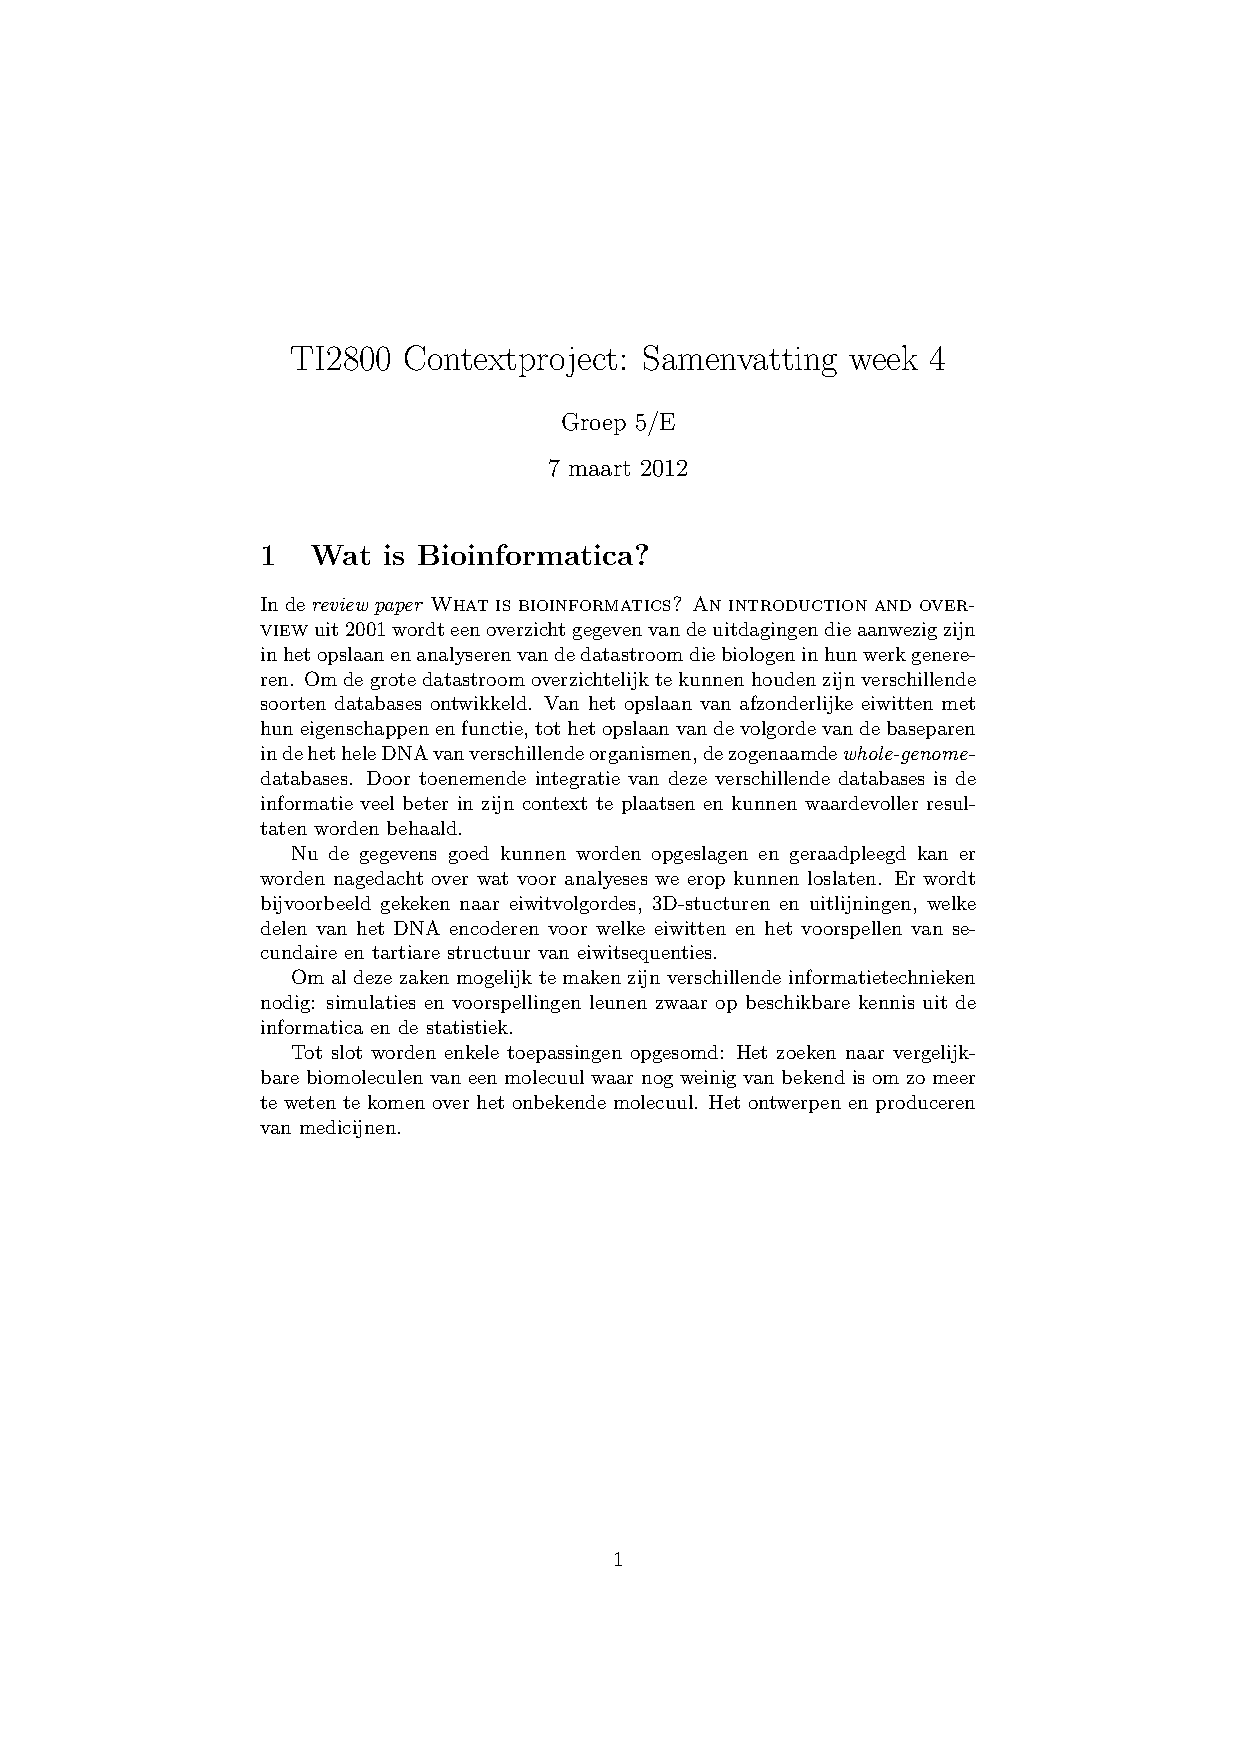
\includepdf{abstracts/lecture-4.pdf}


\end{document}
